\documentclass[12pt,a4paper]{article}
\usepackage[utf8]{inputenc}
\usepackage[english]{babel}
\usepackage{amsmath}
\usepackage{amsfonts}
\usepackage{amssymb}
\usepackage{graphicx}
\usepackage{geometry}
\usepackage{xcolor}
\usepackage{hyperref}
\usepackage{listings}
\usepackage{fancyhdr}
\usepackage{titlesec}
\usepackage{tcolorbox}

\geometry{margin=2.5cm}
\pagestyle{fancy}
\fancyhf{}
\fancyhead[L]{Distributed Systems}
\fancyhead[R]{UNSA}
\fancyfoot[C]{\thepage}

\hypersetup{
    colorlinks=true,
    linkcolor=blue,
    urlcolor=cyan
}

\titleformat{\section}
{\Large\bfseries\color{blue}}
{\thesection.}{1em}{}

\titleformat{\subsection}
{\large\bfseries}
{\thesubsection.}{1em}{}

% Define colors for code
\definecolor{codegray}{rgb}{0.5,0.5,0.5}
\definecolor{codepurple}{rgb}{0.58,0,0.82}
\definecolor{backcolour}{rgb}{0.95,0.95,0.92}

\lstset{
    backgroundcolor=\color{backcolour},
    commentstyle=\color{codegray},
    keywordstyle=\color{blue},
    numberstyle=\tiny\color{codegray},
    stringstyle=\color{codepurple},
    basicstyle=\ttfamily\small,
    breakatwhitespace=false,
    breaklines=true,
    captionpos=b,
    keepspaces=true,
    numbers=left,
    numbersep=5pt,
    showspaces=false,
    showstringspaces=false,
    showtabs=false,
    tabsize=2,
    frame=single
}

\begin{document}

% --- COVER PAGE ---
\begin{titlepage}
    \centering
    \vspace*{1cm}
    
    {\huge\bfseries NATIONAL UNIVERSITY OF SAN AGUSTÍN \par}
    \vspace{0.5cm}
    
    {\Large\bfseries FACULTY OF PRODUCTION AND SERVICES ENGINEERING \par}
    \vspace{0.5cm}
    
    {\large\bfseries PROFESSIONAL SCHOOL OF SYSTEMS ENGINEERING \par}
    
    \vfill
    
    \begin{figure}[h]
        \centering
        
\includegraphics[width=0.22\textwidth]{imagenes/logo_unsa.png}
        \par \vspace{0.5cm}
    \end{figure}
    
    \vfill
    
    {\Large\bfseries INSTALLATION AND DEPLOYMENT GUIDE: \par}
    {\LARGE\bfseries DISTRIBUTED RPC SYSTEM (FLASK + RABBITMQ) \par}
    
    \vfill
    
    \begin{flushleft}
        \textbf{Professor:} Jesús Martín Silva Fernández \\
        \textbf{Course:} Distributed Systems \\
        \textbf{Date:} May 06, 2026
    \end{flushleft}
    
    \vspace{1cm}
    
    \begin{flushright}
        \textbf{Team Members:} \\
        Larico Rodriguez, Bryan Fernando \\
        Maldonado Vilca, Victor Gonzalo \\
        Quispe Huaman, Rodrigo Ferdinand \\
        Salas Aguilar, Juan Victor
    \end{flushright}
    
    \vfill
    
    {\large Arequipa - Peru \par}
\end{titlepage}

\newpage
\tableofcontents
\newpage

\section{System Description}

This project consists of the implementation of the \textbf{Remote Procedure Call (RPC)} pattern using \textbf{Flask} as the HTTP client/server framework and \textbf{RabbitMQ} (through CloudAMQP) as the message broker.

The system is designed to be deployed on \textbf{Render.com} using two independent components that communicate exclusively through message queues.

The RPC pattern allows a program to invoke remote procedures as if they were local functions. In this project, RabbitMQ acts as the messaging intermediary, enabling decoupling between the client and the worker to improve scalability and fault tolerance.

\section{System Architecture}

The data flow follows an asynchronous model where the broker acts as an intermediary:

\begin{enumerate}
    \item The user sends a request to the \textbf{Flask Server}.
    \item Flask publishes the task to the \texttt{rpc\_queue} in \textbf{CloudAMQP}.
    \item The \textbf{Worker} consumes the message, processes the information (uppercase conversion), and returns the result.
    \item The client retrieves the result and displays it to the user.
\end{enumerate}

\begin{figure}[h]
    \centering
    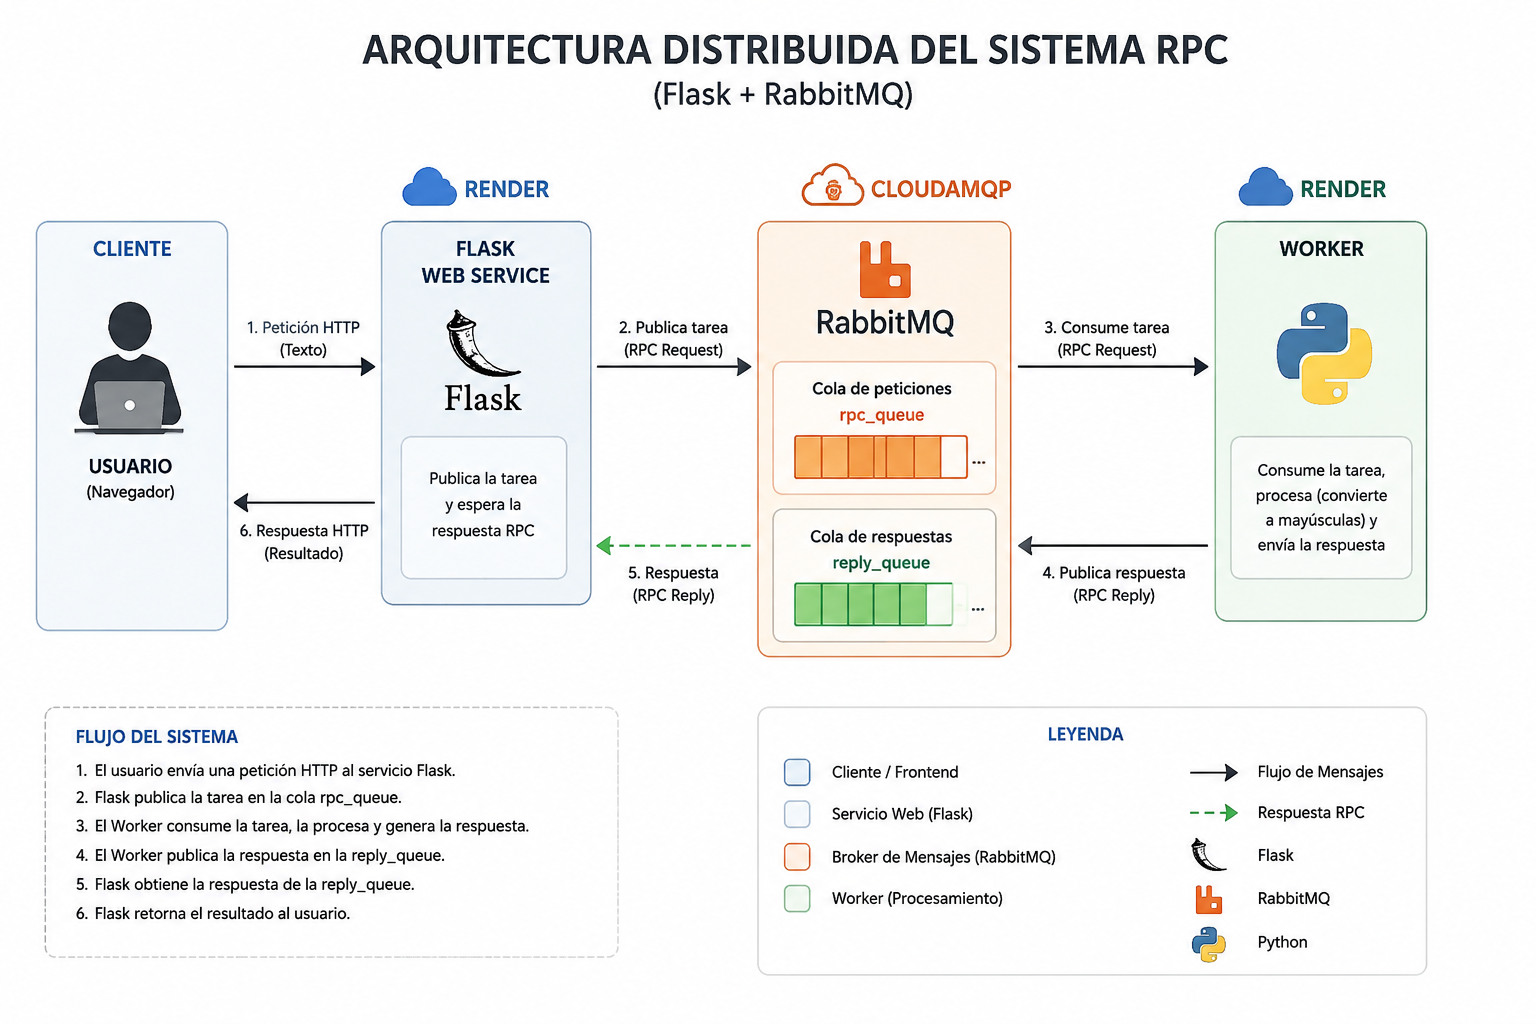
\includegraphics[width=0.85\textwidth]{imagenes/arquitectura.png}
    \caption{Distributed architecture of the RPC system}
\end{figure}

\section{Prerequisites}

To run the system correctly, ensure you have the following:

\begin{itemize}
    \item Python 3.9 or higher.
    \item An active account on \href{https://render.com}{Render.com}.
    \item A free Little Lemur instance on \href{https://cloudamqp.com}{CloudAMQP}.
    \item Git installed on your system.
\end{itemize}

\section{Technologies Used}

\begin{itemize}
    \item Python 3.11
    \item Flask
    \item RabbitMQ
    \item CloudAMQP
    \item Render.com
    \item Gunicorn
    \item AMQPStorm
\end{itemize}

\section{Local Installation and Configuration}

\subsection{Clone the Repository}

\begin{lstlisting}[language=bash]
git clone https://github.com/Victor-Gonzalo-Maldonado-Vilca/Sistemas_Distribuidos_RPC.git
cd Sistemas_Distribuidos_RPC
\end{lstlisting}

\subsection{Development Environment}

Create a virtual environment to isolate dependencies:

\begin{lstlisting}[language=bash]
python -m venv venv

# Activate on Linux/Mac
source venv/bin/activate

# Activate on Windows
venv\Scripts\activate
\end{lstlisting}

Install the required packages:

\begin{lstlisting}[language=bash]
pip install -r requirements.txt
\end{lstlisting}

\section{RabbitMQ Configuration (CloudAMQP)}

\begin{enumerate}
    \item Access your CloudAMQP dashboard.
    \item Copy the \textbf{AMQP URL}.
    \item Replace the value of the \texttt{URL\_NUBE} variable in the files:
    \begin{itemize}
        \item \texttt{worker.py}
        \item \texttt{amqpstorm\_threaded\_rpc\_client.py}
    \end{itemize}
\end{enumerate}

\section{Deployment on Render.com}

For cloud deployment, it is essential to configure two separate services to support the distributed architecture.

\subsection{Service 1: Flask Web Service}

\begin{itemize}
    \item \textbf{Build Command:} \texttt{pip install -r requirements.txt}
    \item \textbf{Start Command:} \texttt{gunicorn amqpstorm\_threaded\_rpc\_client:app}
\end{itemize}

\subsection{Service 2: Worker Service}

Due to Render free-tier limitations, the Worker was deployed as a \textbf{Web Service} configured to listen on port \texttt{10000} using a lightweight dummy HTTP server to prevent Render from stopping the process.

\begin{itemize}
    \item \textbf{Start Command:} \texttt{python worker.py}
\end{itemize}

\section{Troubleshooting}

\begin{itemize}
    \item \textbf{Timeout Error:} If a timeout occurs, verify that the Worker service is in the \texttt{Live} state. Render free-tier services may enter sleep mode after 15 minutes of inactivity.
    
    \item \textbf{Connection Error:} Ensure that the CloudAMQP URL is correct and does not contain invalid characters.
\end{itemize}

\begin{tcolorbox}[colback=yellow!10]
Render free-tier services automatically enter sleep mode after approximately 15 minutes of inactivity.
\end{tcolorbox}

\section{Conclusions}

\begin{itemize}
    \item A distributed RPC-based system was successfully implemented.
    
    \item RabbitMQ enabled decoupled communication between the client and the worker service.
    
    \item Deployment on Render demonstrated the feasibility of cloud-based distributed architectures.
    
    \item The system can be easily scaled by adding multiple worker instances.
\end{itemize}

\section{References}

\begin{itemize}
    \item RabbitMQ Documentation: \url{https://www.rabbitmq.com/}
    
    \item Flask Documentation: \url{https://flask.palletsprojects.com/}
    
    \item Render Documentation: \url{https://render.com/docs}
    
    \item CloudAMQP Documentation: \url{https://www.cloudamqp.com/docs/}
\end{itemize}

\end{document}